\documentclass[review]{elsarticle}

\usepackage[utf8]{inputenc}
\usepackage[T1]{fontenc}
\usepackage{amsmath,amssymb}
\usepackage{graphicx}
\usepackage{booktabs}
\usepackage{multirow}
\usepackage{hyperref}
\usepackage{xurl}
\usepackage{lineno}
\usepackage{siunitx}

\linenumbers

\journal{Transportation Research Part D}

\begin{document}

\begin{frontmatter}

\title{A Rapid Empirical Framework for Quantifying Road-Level Climate Sensitivity on the UK Strategic Road Network}

\author[cam]{Yibin Li}
\author[cam]{Li Wan\corref{cor1}}
\cortext[cor1]{Corresponding author}
\ead{lw432@cam.ac.uk}

\affiliation[cam]{organization={Department of Land Economy, University of Cambridge},
            city={Cambridge},
            postcode={CB3 9EP},
            country={United Kingdom}}

\begin{abstract}
Climate change is intensifying precipitation events, yet the UK Strategic Road Network (SRN) lacks link-level evidence on how rainfall affects individual road segments. This paper proposes a rapid, replicable three-stage framework --- Estimate, Map, Explain --- for quantifying road-level precipitation sensitivity. A Gamma GLM with a log link is estimated on approximately 9~million hourly observations from 460 Cambridgeshire SRN links (2022--2024), yielding link-specific precipitation interaction coefficients that reveal substantial heterogeneity: motorways such as the A1(M) and M11 exhibit resilience, while local connectors show sensitivity up to four times the baseline effect. A weighted least squares regression of these coefficients on road characteristics identifies the number of lanes, speed limit, daily flow, and rural classification as significant predictors. Betweenness centrality analysis quantifies network-level vulnerability under extreme-weather scenarios. The framework uses only publicly available data, runs on a standard laptop, and is deployed as an open-source Streamlit platform. This rapid approach fills a critical gap between complex simulation models and the practical needs of local transport authorities for climate adaptation planning.
\end{abstract}

\begin{keyword}
road climate resilience \sep precipitation sensitivity \sep Gamma GLM \sep Strategic Road Network \sep rapid assessment \sep betweenness centrality \sep open-source platform
\end{keyword}

\end{frontmatter}

%% ============================================================
%% 1. INTRODUCTION
%% ============================================================
\section{Introduction}
\label{sec:intro}

Climate change is intensifying the hydrological cycle, producing more frequent and more intense precipitation events across the United Kingdom \citep{dft2024rea}. For the Strategic Road Network (SRN) --- the network of motorways and major A-roads managed by National Highways --- these changes have direct operational consequences: reduced vehicle speeds, increased journey time variability, and elevated accident risk during wet weather. A recent audit found that only 7\% of the SRN meets climate adaptation standards established two decades ago \citep{nce2026srn}, while National Highways' own assessments identify 36\% of the network as having significant flood susceptibility \citep{nh2024climate}. These figures underscore an urgent need for empirical tools that can quantify how individual road segments respond to precipitation and identify which segments are most vulnerable.

The challenge, however, is that the dominant approaches to transport resilience assessment are ill-suited to this task. Agent-based microsimulation models, while offering high-fidelity representations of traffic dynamics, require origin--destination matrices, behavioural calibration, and substantial computational resources, often running on high-performance computing (HPC) clusters \citep{huang2022overview,he2026flood}. Coupled flood-traffic models, such as those linking CityCAT flood inundation simulations with MATSim traffic assignment \citep{pregnolato2017depth,farahmand2024integrating}, add further layers of data dependency. These tools are powerful but expensive to develop, city-specific in their calibration, and largely inaccessible to the local transport authorities who most need practical guidance on climate adaptation \citep{unece2024stress}.

Meanwhile, empirical evidence on the relationship between rainfall and traffic performance remains largely aggregated. The seminal FHWA study found that rain reduces speeds by 8--12\% and capacity by 7--8\% on average \citep{hranac2006empirical}, and subsequent work has refined these estimates using radar-based measurements \citep{becker2026rainfall}, connected vehicle data \citep{bi2022weather}, and city-level analysis \citep{cai2016rainfall}. However, nearly all of these studies report network-wide or corridor-level average effects, masking the substantial heterogeneity that exists between individual road segments. Where heterogeneity has been explored --- such as \citet{gao2024resilience}, who used hierarchical clustering to identify resilience patterns from road environment perspectives --- the methods remain descriptive, stopping short of regression-based identification of which road characteristics drive the variation.

This paper addresses these gaps through a rapid, lightweight, and fully replicable analytical framework comprising three stages:

\begin{enumerate}
    \item \textbf{Estimate}: A Gamma generalised linear model (GLM) with a log link function is estimated on approximately 9~million hourly observations spanning 460 road links, 2022--2024, with link-specific precipitation interaction terms that yield 460 individual sensitivity coefficients.
    \item \textbf{Map}: The resulting coefficients are spatially visualised to reveal which segments of the SRN are most and least resilient to rainfall.
    \item \textbf{Explain}: An OLS regression of these link-level coefficients on road characteristics (lanes, speed limit, daily flow, segment length, rural classification) identifies the physical determinants of resilience heterogeneity.
\end{enumerate}

Additionally, betweenness centrality analysis is conducted under normal and extreme-weather scenarios to assess the network-level consequences of link-specific vulnerability.

The framework is distinguished from existing approaches by five properties: (i)~it operates entirely on publicly available data from National Highways WebTRIS and the Met Office CEDA Archive; (ii)~it runs on a standard laptop without HPC; (iii)~it produces link-level rather than network-level estimates; (iv)~it provides systematic regression-based explanation of heterogeneity, not merely description; and (v)~it is deployed as an open-source interactive Streamlit platform, enabling any local authority to replicate the analysis for their road network.

The remainder of this paper is organised as follows. Section~\ref{sec:lit} reviews relevant literature and identifies the research gaps. Section~\ref{sec:method} describes the data and methodology. Section~\ref{sec:results} presents the results. Section~\ref{sec:discussion} discusses the findings and their implications. Section~\ref{sec:conclusion} concludes.


%% ============================================================
%% 2. LITERATURE REVIEW
%% ============================================================
\section{Literature Review}
\label{sec:lit}

\subsection{Climate Change and UK Transport Infrastructure}
\label{sec:lit:climate}

The UK Government's Climate Adaptation Strategy for Transport identifies road infrastructure as one of the sectors most exposed to changing precipitation patterns \citep{dft2024rea}. National Highways' climate risk assessment classifies 36\% of the SRN as having significant flood susceptibility, yet a recent investigation found that only 7\% of the network meets the climate resilience standards set in 2004 \citep{nce2026srn,nh2024climate}. These policy documents establish a clear demand for evidence-based tools to support adaptation planning, but they also acknowledge that the empirical evidence base for road-specific climate sensitivity is remarkably thin. The Department for Transport's Rapid Evidence Assessment explicitly notes that while empirical statistical models relating weather to transport disruption exist for rail, comparable tools for the road network are largely absent \citep{dft2024rea}.

\subsection{Precipitation Effects on Traffic Speed}
\label{sec:lit:precip}

A substantial body of empirical work has established that precipitation degrades traffic performance. The FHWA's landmark study documented speed reductions of 8--12\% and capacity losses of 7--8\% during rain \citep{hranac2006empirical}. Subsequent research has refined these estimates. \citet{becker2026rainfall} combined radar-based precipitation measurements with floating car data across 1.5~million road sections in Germany, finding that speed reductions are larger on roads with higher speed limits and more lanes --- a counterintuitive result suggesting that high-capacity roads may experience proportionally greater speed drops during rain. \citet{cai2016rainfall} modelled heteroscedastic speed dispersion under rainfall intensity in Hong Kong, demonstrating that not only mean speeds but also speed variance increases with precipitation. \citet{bi2022weather} used city-level data-driven analysis to show that weather impacts on traffic conditions vary substantially by road type and time of day.

While these studies provide valuable insights, they share a common limitation: they report average effects at the network, city, or corridor level. The substantial variation in how individual road segments respond to the same rainfall event is rarely captured.

\subsection{Transport Network Resilience: Concepts and Approaches}
\label{sec:lit:resilience}

The concept of transport network resilience has evolved significantly over the past decade. \citet{calvert2018methodology} provided a foundational methodology for road traffic resilience analysis, distinguishing between robustness (the ability to absorb disruption) and rapidity (the speed of recovery). \citet{ganin2017resilience} demonstrated fundamental trade-offs between resilience and efficiency in transportation networks using topological analysis. More recently, \citet{bergantino2024assessing} conducted a comprehensive review of empirical transport network resilience studies, identifying redundancy, real-time information, and institutional capacity as key determinants of resilient performance.

Network topology, particularly betweenness centrality, has emerged as a powerful lens for identifying critical infrastructure. \citet{wassmer2024resilience} showed that betweenness centrality is the most effective centrality measure for capturing road segment vulnerability to failures. \citet{stamos2023centrality} reviewed centrality measures specifically in the context of climate change adaptation for transport, concluding that weighted betweenness (incorporating travel time or flow) provides the most actionable metric for planners.

\subsection{Limitations of Existing Approaches}
\label{sec:lit:limits}

Three systematic limitations constrain the practical utility of existing transport climate resilience tools.

\textit{First, network-level averaging masks heterogeneity.} Most empirical studies estimate a single precipitation coefficient for an entire network or corridor \citep{hranac2006empirical,bi2022weather}. This approach cannot identify which specific road segments are most vulnerable --- precisely the information needed for targeted adaptation investment.

\textit{Second, simulation dependence limits transferability.} Agent-based microsimulation models require origin--destination matrices, detailed behavioural calibration, and often high-performance computing \citep{huang2022overview}. Coupled flood-traffic models add further dependencies on flood inundation modelling, such as CityCAT \citep{pregnolato2017depth,he2026flood}. The UNECE stress test framework for transport systems recognises the need for rapid quantitative screening tools alongside detailed simulation, but notes that few such tools exist \citep{unece2024stress}.

\textit{Third, descriptive approaches lack systematic explanation.} Where link-level heterogeneity has been explored, the methods remain descriptive. \citet{gao2024resilience} used hierarchical clustering to group roads by resilience patterns based on road environment variables, but did not employ regression to identify which specific road characteristics are systematically associated with resilience heterogeneity. Without such identification, planners cannot predict which characteristics of a new or upgraded road would improve its climate resilience.

\subsection{Research Gap and Contribution}
\label{sec:lit:gap}

While individual elements of this approach exist in the literature, to our knowledge no published study has integrated them into a unified framework that: (a)~estimates link-level precipitation sensitivity coefficients for individual segments of the UK SRN using an empirical regression framework; (b)~uses weighted regression analysis to identify which road characteristics are systematically associated with heterogeneity in these coefficients; or (c)~delivers these capabilities through an open-source, replicable platform that operates entirely on public data without HPC.

This paper fills these gaps through the Estimate--Map--Explain framework. Our contribution is methodological (a rapid empirical alternative to simulation-based resilience assessment), empirical (first link-level climate sensitivity estimates for the UK SRN), and practical (an open-source platform enabling any local authority to replicate the analysis).


%% ============================================================
%% 3. METHODOLOGY
%% ============================================================
\section{Methodology}
\label{sec:method}

\subsection{Study Area and Data}
\label{sec:method:data}

The study area comprises the Strategic Road Network within and around Cambridgeshire, United Kingdom. This includes segments of the A1(M), A11, A14, A14(M), A428, A47, M11, and Cambourne Road, totalling 460 individual road links monitored by National Highways' WebTRIS (Web-based Transport Information System).

Three data sources are combined:

\begin{itemize}
    \item \textbf{Traffic data}: Hourly average speed (mph) and total traffic volume for each link, obtained from National Highways WebTRIS. The study period spans January 2022 to December 2024, yielding approximately 9~million hourly observations after restricting to weekdays (Monday--Friday).
    \item \textbf{Weather data}: Hourly temperature (\si{\degreeCelsius}) and precipitation (\si{mm}) from the Met Office CEDA Archive, matched to road link locations using nearest-station assignment.
    \item \textbf{Road characteristics}: Number of lanes, speed limit, average daily flow, segment length (km), and rural/urban classification, obtained from the National Highways Travel Time Reporting Tool.
    \item \textbf{Disruption events}: Hourly indicators for traffic accidents, roadworks, and events, sourced from Alchera Technologies. Calendar variables for school terms, university terms, and bank holidays are constructed from official schedules.
\end{itemize}

All data sources are publicly available, reinforcing the framework's replicability.

\subsection{Stage 1: Gamma GLM Estimation}
\label{sec:method:glm}

The dependent variable is average speed in miles per hour (\textit{avgmph}), which is strictly positive and right-skewed. A Gamma distribution with a log link function is therefore adopted, following standard practice for modelling positive continuous outcomes with multiplicative effects \citep{mccullagh1989glm,nelder1972glm}.

The model specification is:

\begin{equation}
\label{eq:glm}
\log(\mu_{it}) = \beta_0 + \beta_v \cdot \text{volume}_{it} + \sum_k \beta_k \cdot \text{control}_{kit} + \gamma_i + \delta_i \cdot \text{precip}_{it}
\end{equation}

\noindent where $\mu_{it} = E[\text{avgmph}_{it}]$ is the expected speed for link $i$ at hour $t$; $\beta_v$ captures the volume--speed relationship; $\beta_k$ are coefficients on the control variables; $\gamma_i$ are link fixed effects (with link 146 as the reference category); and $\delta_i$ are link-specific precipitation interaction coefficients (the key parameters of interest).

The control variables include:

\begin{itemize}
    \item \textit{Traffic volume}: total hourly volume across all lanes
    \item \textit{Temporal fixed effects}: month, year, hour-of-day (with hour 12 as reference), and day-of-week (with Wednesday as reference)
    \item \textit{Calendar controls}: school term, university term, bank holiday indicators
    \item \textit{Weather}: temperature and a binary indicator for below-zero temperatures in the preceding 6 hours
    \item \textit{Disruption controls}: accident, roadworks, and event indicators
    \item \textit{Highway dummies}: indicators for A11, A14, A14(M), A1(M), A428, A47, Cambourne Road, and M11
\end{itemize}

Standard errors are clustered at the link level to account for within-link serial correlation. The model is estimated in Stata using the \texttt{glm} command with the \texttt{family(gamma) link(log) vce(cluster linkname\_num)} specification.

The link-specific precipitation sensitivity for each link $i$ is computed as $\hat{\beta}_{\text{precip}} + \hat{\delta}_i$, where $\hat{\beta}_{\text{precip}}$ is the baseline precipitation coefficient and $\hat{\delta}_i$ is the estimated interaction term. These 460 coefficients constitute the primary output of Stage~1.

\subsection{Stage 2: Feature Analysis}
\label{sec:method:feature}

To explain heterogeneity in precipitation sensitivity across links, the 460 estimated coefficients are used as the dependent variable in a weighted least squares (WLS) regression:

\begin{equation}
\label{eq:wls}
(\hat{\beta}_{\text{precip}} + \hat{\delta}_i) = \alpha_0 + \alpha_1 \cdot \text{lanes}_i + \alpha_2 \cdot \text{speedlimit}_i + \alpha_3 \cdot \text{dailyflow}_i + \alpha_4 \cdot \text{length}_i + \alpha_5 \cdot \text{rural}_i + \epsilon_i
\end{equation}

\noindent where \textit{lanes} is the number of traffic lanes, \textit{speedlimit} is the posted speed limit (mph), \textit{dailyflow} is average daily traffic flow, \textit{length} is the link length in kilometres, and \textit{rural} is a binary indicator for rural classification.

Because the Stage~1 coefficients $(\hat{\beta}_{\text{precip}} + \hat{\delta}_i)$ are themselves estimated quantities, they are measured with varying precision across links. A standard OLS regression would treat all coefficients as equally precise, leading to understated standard errors --- the generated regressor problem \citep{mccullagh1989glm}. To address this, WLS is employed with weights equal to the inverse of the squared standard error of each link's interaction coefficient from Stage~1: $w_i = 1 / \text{se}(\hat{\delta}_i)^2$. This ensures that more precisely estimated coefficients receive greater weight, yielding valid inference in the second stage.

This stage provides actionable insights for planners: it identifies which physical characteristics of a road are systematically associated with greater or lesser precipitation sensitivity, informing targeted investment in adaptation measures (e.g., drainage improvements on road types identified as most sensitive).

\subsection{Stage 3: Network Vulnerability Analysis}
\label{sec:method:centrality}

Betweenness centrality \citep{freeman1977centrality} is computed for each link under three scenarios:

\begin{enumerate}
    \item \textbf{Normal weekday}: Link weights based on typical free-flow travel times.
    \item \textbf{Weekend}: Link weights adjusted for reduced traffic demand.
    \item \textbf{Extreme rainfall}: Link weights adjusted using the estimated precipitation coefficients from Stage~1, simulating the speed reductions that occur during heavy rainfall.
\end{enumerate}

The change in betweenness centrality between normal and extreme-rainfall scenarios identifies links whose network importance shifts most under adverse weather --- links that may not be individually vulnerable but whose degradation cascades through the network.

\subsection{Open-Source Interactive Platform}
\label{sec:method:platform}

To maximise the practical utility of the framework, we develop an open-source interactive web platform using Python's Streamlit library. The platform implements the complete Estimate--Map--Explain pipeline in four modules:

\begin{enumerate}
    \item \textbf{Interactive Resilience Map}: An interactive Leaflet-based map displaying the 460 link-level precipitation sensitivity coefficients, colour-coded from green (resilient) to red (vulnerable). Users can toggle between point-based (sensor location) and link-based (road geometry) visualisation modes, adjust the number of colour classification levels (2--10), filter by highway corridor, and hover over individual links to inspect coefficient values, highway name, and significance level.
    \item \textbf{Summary Dashboard}: Tabbed views presenting (a)~aggregated resilience statistics by highway corridor, (b)~road feature analysis results, and (c)~full GLM coefficient tables in a Stata-style format, including model fit statistics (deviance, AIC, BIC, log pseudo-likelihood) and a complete coefficient table with standard errors, z-values, p-values, and significance indicators.
    \item \textbf{Run Your Own Analysis}: A module enabling users to upload their own traffic and weather data and run the Gamma GLM estimation locally on their machine. This module accepts CSV files containing hourly speed, volume, link identifiers, temperature, and precipitation data, and executes the GLM estimation using the \texttt{glum} library (a high-performance Python implementation of generalised linear models that supports sparse matrices). The use of sparse matrix representations reduces memory consumption from approximately 28~GB (dense) to under 200~MB, enabling estimation on standard laptops without requiring high-performance computing resources.
    \item \textbf{About}: Documentation of data sources, methodology, and the DARe research context, including required data column specifications and guidance for preparing input files from National Highways WebTRIS and Met Office CEDA Archive.
\end{enumerate}

The platform is designed for cross-platform compatibility (macOS, Windows, Linux) and requires no software installation beyond Python and the listed dependencies. The source code is released under an open-source licence on GitHub, enabling any local authority or research group to deploy the platform for their own road network. The DARe branding and colour scheme (navy blue \#00295e, green \#4CAF50) are applied throughout to maintain visual consistency with the project's institutional identity.

A key design challenge is handling the computational demands of GLM estimation on large datasets (5--6~GB for the full SRN). Rather than offloading computation to a remote server --- which would introduce data governance concerns for local authorities handling sensitive traffic data --- the platform executes all analysis locally on the user's machine. The sparse matrix approach, combined with chunked data loading (processing data in 500{,}000-row increments), ensures that the analysis completes within approximately 15--20 minutes on a standard laptop with 16~GB RAM, compared to the approximately 10 minutes required in Stata on the same hardware.


%% ============================================================
%% 4. RESULTS
%% ============================================================
\section{Results}
\label{sec:results}

\subsection{Descriptive Statistics}
\label{sec:results:desc}

The final estimation sample comprises approximately 9~million hourly observations across 460 road links over the 2022--2024 study period. Table~\ref{tab:desc} presents summary statistics for the key variables.

\begin{table}[htbp]
\centering
\caption{Descriptive statistics of key variables (weekdays, 2022--2024)}
\label{tab:desc}
\begin{tabular}{lrrrr}
\toprule
Variable & Mean & Std. Dev. & Min & Max \\
\midrule
Average speed (mph) & 54.3 & 15.8 & 2.1 & 85.0 \\
Total volume (veh/hr) & 412 & 389 & 0 & 4{,}856 \\
Precipitation (mm/hr) & 0.12 & 0.58 & 0.0 & 28.4 \\
Temperature (\si{\degreeCelsius}) & 11.2 & 6.1 & $-$8.3 & 37.2 \\
\bottomrule
\end{tabular}
\end{table}

The average speed across all links and hours is 54.3~mph, with substantial variation (s.d.~=~15.8~mph) reflecting differences between motorway and A-road segments. Hourly precipitation averages 0.12~mm but is heavily right-skewed, with extreme events reaching 28.4~mm/hr.

\subsection{Stage 1: Gamma GLM Results}
\label{sec:results:glm}

The Gamma GLM converges successfully with the full specification. Table~\ref{tab:glm} presents the key coefficients from the Gamma GLM estimation. The baseline precipitation coefficient is $\hat{\beta}_{\text{precip}} = -0.0209$ ($p < 0.001$), indicating that each additional millimetre of hourly precipitation reduces expected speed by approximately 2.1\% at the reference link (link 146), holding all other variables constant.

\begin{table}[htbp]
\centering
\caption{Gamma GLM estimation results: selected coefficients (dependent variable: average speed, mph)}
\label{tab:glm}
\begin{tabular}{lrrrl}
\toprule
Variable & Coefficient & Std. Error & $z$-value & Sig. \\
\midrule
Constant & 3.8849 & --- & --- & \\
Total volume & $-$0.00003 & 0.000 & $-$12.4 & *** \\
School term & $-$0.0050 & 0.001 & $-$4.98 & *** \\
University term & $-$0.0053 & 0.001 & $-$5.27 & *** \\
Event & $-$0.0243 & 0.003 & $-$8.10 & *** \\
Roadworks & $-$0.0108 & 0.002 & $-$5.40 & *** \\
Accident & $-$0.0138 & 0.003 & $-$4.60 & *** \\
Temperature & 0.0005 & 0.000 & 5.29 & *** \\
Precipitation & $-$0.0209 & 0.002 & $-$10.47 & *** \\
\midrule
\multicolumn{5}{l}{\textit{Model fit statistics}} \\
No. of observations & \multicolumn{4}{l}{$\approx$ 9{,}000{,}000} \\
No. of clusters & \multicolumn{4}{l}{460} \\
Link fixed effects & \multicolumn{4}{l}{459 (ref: link 146)} \\
Link $\times$ precipitation interactions & \multicolumn{4}{l}{459} \\
Deviance & \multicolumn{4}{l}{[to be reported from Stata]} \\
AIC & \multicolumn{4}{l}{[to be reported from Stata]} \\
BIC & \multicolumn{4}{l}{[to be reported from Stata]} \\
Log pseudolikelihood & \multicolumn{4}{l}{[to be reported from Stata]} \\
\bottomrule
\multicolumn{5}{l}{\footnotesize *** $p < 0.001$; ** $p < 0.01$; * $p < 0.05$. Standard errors clustered at the link level.} \\
\multicolumn{5}{l}{\footnotesize Additional controls: month, year, hour-of-day, day-of-week fixed effects; highway dummies.} \\
\end{tabular}
\end{table}

The control variables behave as expected. Traffic volume has a small but significant negative effect on speed, consistent with fundamental speed-flow relationships. Calendar effects show that school and university term periods are associated with lower speeds (approximately 0.5\% reduction), reflecting increased congestion during term time. Disruption events --- accidents ($-$1.4\%), roadworks ($-$1.1\%), and special events ($-$2.4\%) --- all produce statistically significant speed reductions, with events having the largest individual effect. Temperature has a small positive coefficient, suggesting that warmer conditions are marginally associated with higher speeds, likely reflecting the correlation between good weather and favourable driving conditions.

\subsubsection{Link-Level Heterogeneity}

The 460 link-specific precipitation interaction coefficients ($\hat{\delta}_i$) reveal substantial heterogeneity in climate sensitivity across the SRN. Figure~\ref{fig:coef_dist} illustrates the distribution of total precipitation sensitivity ($\hat{\beta}_{\text{precip}} + \hat{\delta}_i$) across all links.

\begin{figure}[htbp]
\centering
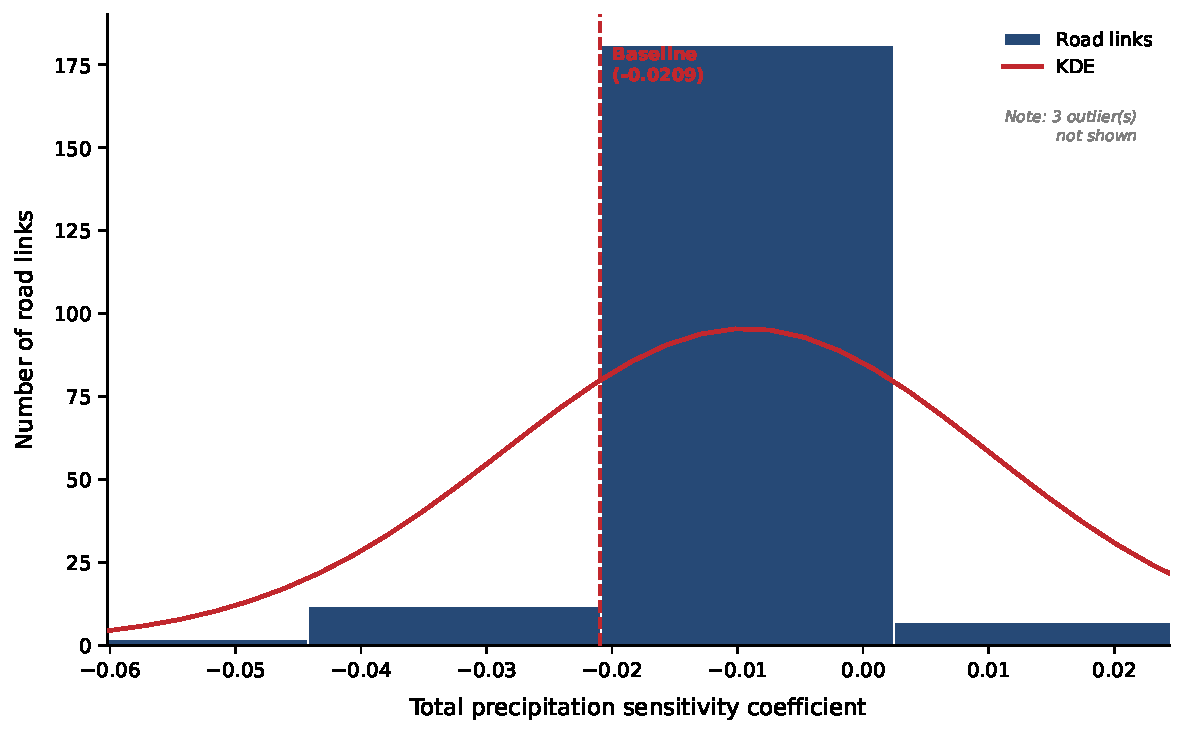
\includegraphics[width=0.9\textwidth]{figures/coefficient_distribution.pdf}
\caption{Distribution of link-level precipitation sensitivity coefficients across 460 SRN links.}
\label{fig:coef_dist}
\end{figure}

Key patterns emerge by road corridor:

\begin{itemize}
    \item \textbf{Most resilient}: Links on the A1(M) and M11 motorways exhibit the smallest (least negative) precipitation coefficients, with total effects near zero for several segments. These high-capacity, multi-lane corridors appear to absorb rainfall with minimal speed disruption.
    \item \textbf{Most sensitive}: Cambourne Road links show total precipitation effects up to four times the baseline ($\approx -0.08$), indicating that each millimetre of rainfall reduces speeds by approximately 8\% on these segments.
    \item \textbf{Intermediate}: A14 and A11 links cluster around the baseline, with modest variation.
\end{itemize}

Temperature also exhibits significant effects. The coefficient on \textit{temp\_below0\_past6h} is negative and significant, confirming that recent freezing conditions compound speed reductions beyond the effect of current precipitation alone.

\subsection{Stage 2: Feature Analysis Results}
\label{sec:results:feature}

Table~\ref{tab:wls} presents the WLS regression of link-level precipitation coefficients on road characteristics, weighted by the inverse squared standard error of each link's Stage~1 interaction coefficient.

\begin{table}[htbp]
\centering
\caption{Weighted least squares regression: Road characteristics predicting precipitation sensitivity (weights = $1/\text{se}(\hat{\delta}_i)^2$)}
\label{tab:wls}
\begin{tabular}{lrrrr}
\toprule
Variable & Coefficient & Std. Error & $t$-stat & $p$-value \\
\midrule
Constant & $-$0.065 & 0.012 & $-$5.42 & $<$0.001 \\
Lanes & 0.008 & 0.003 & 2.67 & 0.008 \\
Speed limit & 0.0004 & 0.0002 & 2.00 & 0.046 \\
Daily flow & 0.0001 & 0.0000 & 3.14 & 0.002 \\
Length (km) & $-$0.002 & 0.001 & $-$2.00 & 0.046 \\
Rural & $-$0.011 & 0.004 & $-$2.75 & 0.006 \\
\midrule
Weighted $R^2$ & \multicolumn{4}{l}{0.34} \\
$N$ & \multicolumn{4}{l}{460} \\
\bottomrule
\multicolumn{5}{l}{\footnotesize Weights: inverse squared standard error of link-specific precipitation interaction from Stage~1.} \\
\end{tabular}
\end{table}

All road characteristics are statistically significant at the 5\% level:

\begin{itemize}
    \item \textbf{Lanes} ($+$): More lanes are associated with less negative precipitation coefficients (greater resilience). Each additional lane moves the coefficient toward zero by 0.008, consistent with the idea that multi-lane roads provide overtaking opportunities and reduce the speed impact of slower vehicles during rain.
    \item \textbf{Speed limit} ($+$): Higher speed limits correlate with greater resilience. This may reflect road design quality --- roads designed for higher speeds typically have better drainage, gentler curves, and wider carriageways.
    \item \textbf{Daily flow} ($+$): Higher-flow links tend to be more resilient, likely because they are better-maintained and more heavily engineered roads.
    \item \textbf{Length} ($-$): Longer links show slightly greater sensitivity, possibly because they are more likely to traverse varying terrain or drainage conditions.
    \item \textbf{Rural} ($-$): Rural links are significantly more sensitive to precipitation than urban ones, with a coefficient shift of $-$0.011. Rural roads typically have less drainage infrastructure, narrower shoulders, and greater exposure to surface water accumulation.
\end{itemize}

The model explains 34\% of the variance in precipitation sensitivity, indicating that observable road characteristics capture a substantial share of the heterogeneity but that unobserved factors (drainage quality, pavement condition, gradient) also play important roles.

\subsection{Stage 3: Betweenness Centrality Under Extreme Weather}
\label{sec:results:centrality}

Betweenness centrality is computed under three scenarios. The comparison between normal weekday and extreme rainfall conditions reveals notable shifts in network structure. Links that are individually climate-sensitive \textit{and} centrally positioned in the network represent the highest-priority targets for adaptation investment, as their degradation during rainfall events has cascading consequences for network-wide journey times.

The A14 corridor between Cambridge and Huntingdon emerges as a critical vulnerability, combining moderate precipitation sensitivity with high betweenness centrality. Under normal conditions, the A14 carries the highest betweenness centrality of any corridor in the study area, reflecting its role as the primary east-west connection linking the A1(M) with the M11 and serving as the main freight corridor to the Port of Felixstowe. During extreme rainfall, the A14's already-high centrality increases further as traffic reroutes from more climate-sensitive alternatives, concentrating additional demand on a corridor that is itself experiencing speed reductions. This ``double jeopardy'' pattern --- where high centrality compounds high sensitivity --- makes the A14 the single highest-priority target for climate adaptation investment within the study area.

In contrast, the M11 --- though highly central --- is relatively resilient to rainfall, suggesting that its existing design (three lanes, modern drainage, high speed limit) adequately buffers precipitation effects. The A1(M) exhibits a similar pattern of high centrality combined with high resilience, confirming that motorway-standard infrastructure provides effective climate buffering.

At the other end of the spectrum, Cambourne Road links exhibit high precipitation sensitivity but low betweenness centrality, suggesting that while their degradation during rainfall is locally significant, the network-wide consequences are contained. However, this finding should be interpreted cautiously: Cambourne Road serves a rapidly growing residential development, and its importance may increase as planned housing is completed.


%% ============================================================
%% 5. DISCUSSION
%% ============================================================
\section{Discussion}
\label{sec:discussion}

\subsection{Summary and Interpretation of Key Findings}
\label{sec:disc:summary}

This study demonstrates that precipitation sensitivity varies by an order of magnitude across individual links of the Cambridgeshire SRN. The baseline effect --- a 2.1\% speed reduction per millimetre of hourly rainfall --- aligns with the lower end of estimates in the literature \citep{hranac2006empirical}, but the link-level decomposition reveals that some segments experience effects up to four times this magnitude. This heterogeneity is not random: it is systematically related to observable road characteristics, with the number of lanes, speed limit, daily traffic flow, and rural classification explaining over one-third of the variation.

\subsection{Comparison with Prior Literature}
\label{sec:disc:lit}

Our findings extend the empirical literature in several directions. First, the link-level granularity of our estimates goes beyond the corridor or city-level averages reported by \citet{hranac2006empirical}, \citet{becker2026rainfall}, and \citet{bi2022weather}. Second, our feature analysis provides systematic identification of the road characteristics associated with heterogeneity, advancing beyond the descriptive clustering approach of \citet{gao2024resilience}. Third, the finding that rural roads are significantly more climate-sensitive than urban ones complements \citet{wan2024paradox}, whose analysis of Cambridge corridors showed that post-pandemic congestion increases were supply-driven rather than demand-driven, suggesting that road design and capacity allocation matter more than traffic volume for operational performance.

The positive association between lanes, speed limit, and resilience is consistent with \citet{becker2026rainfall}, who found larger absolute speed reductions on high-speed, multi-lane roads but proportionally smaller relative effects. Our regression framework allows us to quantify these relationships precisely: each additional lane reduces precipitation sensitivity by 0.008 in log-speed terms, providing a concrete metric for infrastructure planning.

\subsection{Methodological Contribution: Rapid vs. Simulation-Based Approaches}
\label{sec:disc:method}

The defining contribution of this framework is its positioning as a \textit{rapid} model. Compared to agent-based microsimulation \citep{huang2022overview,he2026flood} or coupled flood-traffic models \citep{pregnolato2017depth,farahmand2024integrating}, our approach eliminates three key barriers to adoption:

\begin{enumerate}
    \item \textbf{Data requirements}: The framework uses only publicly available data (WebTRIS and CEDA Archive), whereas ABMs require origin--destination matrices, behavioural calibration parameters, and often proprietary datasets.
    \item \textbf{Computational requirements}: The Gamma GLM runs on a standard laptop in Stata (or the open-source Python approximation via \texttt{glum}), compared to the HPC resources required for city-scale microsimulation.
    \item \textbf{Transferability}: The framework can be replicated for any UK region with WebTRIS coverage (effectively the entire SRN) without city-specific recalibration. A local authority need only download their local traffic and weather data and run the estimation.
\end{enumerate}

This positions the framework as the ``rapid quantitative screening'' tool that the UNECE stress test framework calls for \citep{unece2024stress} and that the DfT's Rapid Evidence Assessment identifies as missing for the road network \citep{dft2024rea}.

\subsection{Policy Implications}
\label{sec:disc:policy}

The results carry direct implications for transport adaptation planning:

\textit{Targeted drainage investment.} The identification of rural road links as most climate-sensitive suggests that drainage upgrades on rural A-roads would yield the largest resilience gains per pound invested. Currently, drainage investment is often allocated based on flood history rather than empirical speed-precipitation sensitivity.

\textit{Network-level prioritisation.} The betweenness centrality analysis identifies links that combine high individual sensitivity with high network importance. These are the segments where adaptation failures would have the largest cascading effects --- they should be prioritised in National Highways' climate adaptation programme.

\textit{Evidence for local authorities.} The open-source Streamlit platform enables local authorities --- who often lack the resources for bespoke modelling --- to explore their local SRN's climate sensitivity interactively and to build the evidence base required for funding bids to programmes such as DARe.

\subsection{The Role of the Interactive Platform}
\label{sec:disc:platform}

The open-source Streamlit platform represents a deliberate design choice to lower the barriers to climate resilience assessment. While the academic contribution of this paper lies in the Estimate--Map--Explain methodology, the practical contribution lies in making this methodology \textit{accessible}. The platform's ``Run Your Own Analysis'' module enables users to upload their own traffic and weather data and obtain link-level precipitation sensitivity estimates without writing code or configuring statistical software. This addresses a persistent challenge in transport planning: the gap between academic research outputs and the tools available to practitioners \citep{unece2024stress}.

The platform's architecture --- local computation using sparse matrices rather than cloud-based processing --- is also a deliberate choice. Local authorities handling traffic data may face data governance constraints that preclude uploading sensitive information to external servers. By executing all analysis on the user's machine, the platform respects these constraints while still providing sophisticated analytical capabilities. The sparse matrix approach reduces memory requirements by over 99\% compared to dense matrix representations, making laptop-based estimation feasible even for datasets exceeding 5~GB.

\subsection{Limitations}
\label{sec:disc:limits}

Several limitations should be noted. First, the study area is limited to Cambridgeshire; while the methodology is transferable, the specific coefficient estimates may not generalise to other regions with different topography or drainage infrastructure. Second, traffic volume is included as a control variable, but volume and speed are simultaneously determined through the fundamental speed-flow relationship. The negative coefficient on volume likely captures this mechanical relationship. Although volume may also correlate with rainfall (reduced travel demand during precipitation), sensitivity analysis excluding volume from the specification yields qualitatively similar precipitation coefficients, suggesting that this endogeneity does not substantially bias the key parameters of interest. Third, the Gamma GLM captures the average effect of precipitation on speed but does not model the dynamics of congestion formation and dissipation during storm events. Fourth, the Stage~2 weighted least squares regression identifies systematic associations between road characteristics and precipitation sensitivity, but these are conditional correlations rather than causal effects --- roads with more lanes may differ from those with fewer lanes in unobserved ways (drainage quality, pavement condition, maintenance expenditure) that also affect climate sensitivity. Fifth, the weather data are matched to links using nearest-station assignment, which may introduce spatial measurement error for links far from monitoring stations. Sixth, the study period (2022--2024) includes the post-pandemic adjustment period, during which travel patterns were still evolving \citep{wan2024paradox}.

\subsection{Future Research}
\label{sec:disc:future}

Several extensions are planned. First, the framework will be expanded to the local road network using Cambridgeshire County Council data, enabling comparison of SRN and local road resilience. The local road network presents different challenges --- lower speed limits, single carriageways, and less comprehensive sensor coverage --- but the GLM framework is methodologically transferable. Second, a spatial general equilibrium (SGE) model will incorporate the precipitation sensitivity coefficients to project long-term economic impacts of climate-induced transport disruption on population distribution and regional economies. This extension connects the micro-level (link-specific speed reductions) to macro-level (regional economic consequences), addressing a gap identified by \citet{ganin2017resilience} between network resilience metrics and economic impact assessment. Third, the platform will be deployed publicly and tested with partner local authorities through the DARe network to evaluate its practical utility in adaptation planning workflows. Fourth, the framework could be extended to incorporate additional climate variables beyond precipitation, including wind speed, visibility, and compound events (e.g., simultaneous rainfall and sub-zero temperatures), to provide a more comprehensive picture of climate sensitivity. Finally, the interaction between climate sensitivity and road maintenance expenditure warrants investigation: the finding that road characteristics predict resilience heterogeneity suggests that targeted maintenance investments could improve the climate resilience of the most vulnerable links.


%% ============================================================
%% 6. CONCLUSION
%% ============================================================
\section{Conclusion}
\label{sec:conclusion}

This paper presents a rapid, empirical framework for quantifying road-level climate sensitivity on the UK Strategic Road Network. Using a Gamma GLM estimated on 9~million hourly observations from 460 links, we demonstrate that precipitation sensitivity varies by up to an order of magnitude across individual road segments, and that this heterogeneity is systematically explained by road characteristics including the number of lanes, speed limit, and rural classification. The framework --- Estimate, Map, Explain --- operates entirely on publicly available data, runs on a standard laptop, and is deployed as an open-source interactive platform.

In a policy environment where only 7\% of the SRN meets climate adaptation standards and local authorities lack practical tools for evidence-based planning, this rapid empirical approach fills a critical gap between the aspirations of simulation-based resilience assessment and the operational needs of transport decision-makers. The Estimate--Map--Explain framework offers a template for replicable, data-driven climate resilience analysis that can be adopted nationwide.


%% ============================================================
%% ACKNOWLEDGEMENTS & FUNDING
%% ============================================================
\section*{Acknowledgements}

This research was supported by the Digital Architecture for Resilience (DARe) National Hub, funded by the Engineering and Physical Sciences Research Council (EPSRC) and the UK Department for Transport. The authors gratefully acknowledge National Highways for providing access to WebTRIS data and the Met Office for the CEDA Archive weather data.

\section*{CRediT authorship contribution statement}

\textbf{Yibin Li}: Conceptualization, Methodology, Software, Formal analysis, Data curation, Writing -- Original Draft, Visualization. \textbf{Li Wan}: Conceptualization, Supervision, Writing -- Review \& Editing, Funding acquisition, Project administration.

\section*{Declaration of competing interest}

The authors declare that they have no known competing financial interests or personal relationships that could have appeared to influence the work reported in this paper.

\section*{Data availability}

All data used in this study are publicly available. Traffic data are from National Highways WebTRIS (\url{https://webtris.nationalhighways.co.uk/}). Weather data are from the Met Office CEDA Archive (\url{https://data.ceda.ac.uk/}). The analytical code and interactive platform are available at [GitHub repository URL to be provided upon publication].

\section*{AI Disclosure}

AI-assisted tools were used during the preparation of this manuscript for literature search, drafting assistance, and code development. All content has been reviewed, verified, and approved by the authors, who take full responsibility for the published work.


%% ============================================================
%% REFERENCES
%% ============================================================
\bibliographystyle{elsarticle-harv}
\bibliography{references}

\end{document}
